%!TEX root =SpGEMM_Accumulo_HPEC.tex

\section{Discussion}
\label{sDiscussion}

\subsection{TableMult Design Alternatives}

A common Accumulo pattern is to run multiple clients that scan disjoint and continuous table sections in parallel.
We avoid this pattern because it increases client software complexity,
whereas we aim to provide a service within Accumulo that works for any client.
Perhaps more importantly, previous work has shown that table scans 
that do not perform significant iterator processing %filtering or other server-side computation 
bottleneck on communication overhead \emph{at the client} related to Apache Thrift serialization \cite{sawyer2013understanding}.
We gain a chance to eliminate this overhead by moving computation to the server,
though we do not currently do so as we use standard Accumulo Scanners and BatchWriters.

%bridge inner and outer product
We also find room to reconsider the inner product SpGEMM formulation from our initial design
because it has an opposite performance profile as Figure~\ref{fInnerOuterSpectrum} depicts: 
inner product bottlenecks on scanning whereas outer product bottlenecks on writing.
At the expense of multiple passes over input matrices, inner product emits entries more efficiently
in that emitted entries are in order and partial products can sum immediately, 
reducing the number of entries written to Accumulo to the minimum possible.
Outer product reads inputs in a single pass
but emits %entries less efficiently in that entries emit 
entries out of order and 
has little chance to pre-sum partial products, 
instead writing individual partial products to the result table.
Table~\ref{tResultsParams} quantifies the additional number of entries outer product writes
for power law inputs as 2.5 to 3 times that of inner product.
In the worst case, multiplying a fully dense $n \times m$ with an $m \times p$ matrix,
outer product would emit $m$ times more entries than inner product.

\begin{figure}[tbh]
\centering
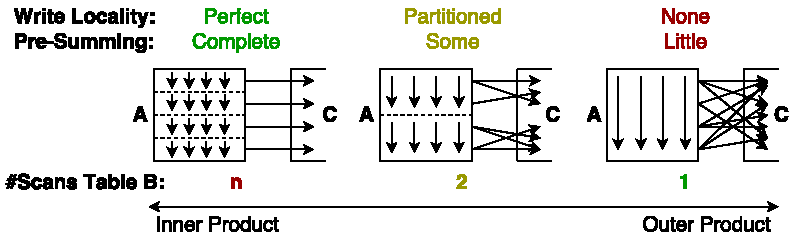
\includegraphics[width=\linewidth]{InnerOuterSpectrum}
\caption{Tradeoffs between Inner and Outer Product}
\label{fInnerOuterSpectrum}
\end{figure}

%LRU cache enables the bridge
Is it possible to blend inner and outer product algorithms and achieve better performance than either method alone?
A definitive answer is future research, though we sketch one possible bridge in Figure~\ref{fInnerOuterSpectrum}.
Suppose we partition the rows of $\matr{A}$ (columns of $\matr{A^\tr}$) into two halves 
and run outer product on each separately.
Each outer product requires one scan over $\matr{B}$ for a total of two passes.
In exchange we increase write locality:
the top half outer product only writes to the top half of $\matr{C}$ and 
the bottom half outer product only writes to the bottom half of $\matr{C}$.
%We could do the same process on table $\matr{B}$ by symmetry.
Selecting the number of partitions along rows of $\matr{A}$ determines
balance between inner product (partitions between every row) and outer product (zero partitions).

A challenge for any hybrid algorithm is mapping it to Accumulo infrastructure.
We chose outer product because it more naturally fits into Accumulo, 
using iterators for one-pass streaming computation, 
BatchWriters to handle unsorted entry emission and Combiners to defer summation.
%Hybrid solutions might consider locality groups or transpose tables to enable column-oriented scanning
%and the distribution of tablets to tablet server cost modeling to 
We may realize greater performance by considering data placement among tablet servers, 
but such a consideration would require accessing and perhaps manipulating
Accumulo's internal state and non-public API.
We suggest this paper's approach as a balance between top performance and implementation stability.


\subsection{TableMult in Algorithms}
Several optimization opportunities exist for TableMult as a primitive in larger algorithms.
Suppose we have a program $\matr{E} = \matr{AB}; \matr{F} = \matr{CD}; \matr{G} = \matr{EF}$.
We would save a round trip to disk if we could mark tables $\matr{E}$ and $\matr{F}$ as 
``temporary tables,'' i.e. tables intermediate to an algorithm that should be held in memory 
and not written to Hadoop if possible.

A \emph{pipelining} optimization streams entries from a TableMult to downstream computations. 
Outer product pipelining is difficult
because it cannot guarantee all partial products for any particular element 
are written to table $\matr{C}$ until it finishes.
Inner product's write locality makes it easier to pipeline.
More ambitiously, a \emph{loop fusion} optimization merges iterator stacks 
for two computations into one. 

Optimizing computation on NoSQL databases is challenging in the general case because
NoSQL databases mostly exclude query planner features 
customary of SQL databases in exchange for raw performance.
NewSQL databases aim in part to achieve the best of both worlds---performance and query planning \cite{grolinger2013data}.
We aspire to make a small step for Accumulo in the direction of NewSQL with current Graphulo research.



\subsection{Related Work} %Analogy to MapReduce with Accumulo Scanners, Iterators and BatchWriters:
%\todo[inline]{Cannon's algorithm, other SpGEMM}
Bulu\c{c} and Gilbert studied message passing algorithms for SpGEMM
such as Sparse SUMMA, most of which use 2D block decompositions \cite{buluc2012parallel}.
Unfortunately, 2D decompositions are difficult in Accumulo 
and message passing even more so.
In this work we use Accumulo's native 1D decomposition along rows 
and no tablet server communication
other than shuffling partial products to tablets of $\matr{C}$ via BatchWriters.


Our outer product method could have been implemented in MapReduce %x\cite{dean2008mapreduce} 
on Hadoop or its successor YARN \cite{vavilapalli2013apache}.
In fact, there is a natural analogy from how we process data in Accumulo to MapReduce:
the map phase scans rows from $\matr{A^\tr}$ and $\matr{B}$
and generates a list of partial products from TwoTableIterator;
the shuffle phase sends partial products to the correct tablet of $\matr{C}$ via BatchWriters;
the reduce phase sums partial products using Accumulo Combiners.
Examining the conditions on which MapReduce outperforms an Accumulo-only solution
is worthy future work.




\section{Conclusions}
\label{sConclusions}

In this work we showcase the design of TableMult, a Graphulo implementation of the 
SpGEMM GraphBLAS linear algebra kernal server-side on Accumulo tables.
We compare inner and outer approaches for SpGEMM and show how outer product is better
suited to the Accumulo iterator environment.
Performance experiments show good weak scaling and hint at strong scaling,
although repeating our experiments on a larger cluster is necessary to confirm.

Current research is to implement the remaining GraphBLAS kernels 
and develop algorithms calling them, % atop the Graphulo library,
ultimately delivering a Graphulo linear algebra library 
as a pattern for server-side computation
to the Accumulo community.
